\documentclass[20pt,landscape]{foils}
\usepackage{amsmath, amssymb, amsthm}
\usepackage{color}
\usepackage{hyperref}
%\usepackage{pause}
\usepackage{graphicx}
\usepackage{epsfig}
%\usepackage{geometry}
%\geometry{headsep=3ex,hscale=0.9}
\newcommand{\bd}{\textbf}
\newcommand{\no}{\noindent}
\newcommand{\un}{\underline}
\newcommand{\bi}{\begin{itemize}}
\newcommand{\ei}{\end{itemize}}
\newcommand{\be}{\begin{enumerate}}
\newcommand{\ee}{\end{enumerate}}
\newcommand{\bc}{\begin{center}}
\newcommand{\ec}{\end{center}}
\newcommand \h {\hspace*{.3in}}
\newcommand{\bul}{\hspace*{.3in}{\textcolor{red}{$\bullet$ \ }}}
\newcommand{\xbar}{\bar{x}}
\rightheader{Stat 330 (Fall 2016): slide set 5}

\begin{document}
\LogoOff

\foilhead[1.3in]{}
\centerline{\LARGE \textcolor{blue}{Slide set 5}}
\vspace{0.3in}
\centerline{\large Stat 330 (Fall 2016)}
\vspace{0.2in}
\centerline{\tiny Last update: \today}
\setcounter{page}{0}

\foilhead[-.8in]{\textcolor{blue}{Conditional Probability}}
\no  {\textcolor{magenta}{Example 1:}  {\textcolor{cyan}{A box has 5 computer chips. Two are defective.  Two chips are  selected from the box, one at a time.}} \\[.1in]
\no 1. {\textcolor{cyan}{Compute the probability that the second chip is defective. }}\\[.1in]
\no Again common sense tells us that $ P(\text{ a chip is defective}) = \frac{2}{5}$.\\[.1in] 
\no Using probability theory, we have \\[.1in]
\no $|\Omega|$ = \# of ways to draw 2 chips (ordered) = (5)(4)=20\\[.1in] 
\no Define event $A =\mbox{the second chip is defective}$\\
 \no $|A|$ = \# of outcomes with second chip defective= (4)(2)=8\\[.1in] 
$$P(\text{ second chip is defective}) = \frac{|A|}{|\Omega|} = \frac{8}{20}=.4.$$
\no 2. {\textcolor{cyan}{If we know that the first chip drawn is good, what is the probability that the second chip is defective?}} 
 

\foilhead[-.7in]{\textcolor{blue}{Conditional Probability (continued)}}
\no When we obtain additional information about a probability experiment, we want to reassess the probabilities of events given the new information.\\[.1in]  
\no {\textcolor{red}{Definition:}} The conditional probability of an event $A$ given an event $B$ is 
$$P(A|B) =\frac{P(A\cap B)}{P(B)},$$
\no \hspace*{1.6in}provided $P(B)\neq 0$.\\[.1in]
\no {\textcolor{magenta}{The above definition makes sense because the conditional probability of $A$ given $B$ is the fraction of outcomes in $B$ that are also in $A$}. \\[.1in]
\no An important implication of the definition is that  
$$ \qquad P(A\cap B) = P(A|B)P(B)= P(B|A)P(A).$$
\no Knowing two of the above probabilities allow us to compute the third.

\foilhead[-.7in]{\textcolor{blue}{Conditional Probability (continued)}}
\no {\textcolor{cyan}{Compute the probability that the second chip is defective given that the first chip is good using the above definition.}}\\[.1in] 
\no Let  $A$=the first chip is good; $B=$ the second chip is defective.\\[.1in]
Now we need to compute $P(B|A)$\\[.15in] 
\no First, we have that $P(A)=\frac{3}{5}$ \\[.15in] 
\no The event $ A\cap B$  is  first chip is good and the second chip is defective.\\[.1in] 
\no The \# of outcomes with first chip is good and the second chip is defective $= (3)(2)$\\[.1in]
\no Thus we have that $P(A\cap B)=\frac{6}{20}$\\[.1in]
\no Thus $$P(B|A) =\frac{P(A\cap B)}{P(A)}=\frac{6/20}{3/5}=.5$$

\foilhead[-.8in]{\textcolor{blue}{ More computer chips...}}
\no {\textcolor{magenta}{Example 2:}}  {\textcolor{cyan}{A box has 500 computer chips with a speed of 400 Mhz and 500 with a speed of 500 Mhz. The numbers of good (G) and defective (D) chips at the two different speeds are as shown below.}} 
\begin{center}{\small
\begin{tabular}{c|c|c|c}
& 400 Mhz & 500 Mhz & \\[.01in]
\hline 
G & 480 & 490 & 970  \\[.01in]
\hline
D & 20 & 10 & 30   \\[.01in] 
\hline
& 500 & 500 & Total=1000    
\end{tabular}}
\end{center}
\no 1. {\textcolor{cyan}{We select a chip at random and observe its speed. What is the probability that the chip is defective given that its speed is 400 Mhz?}}\\[.01in] 
Drawing a chip at random has the following probabilities:\\[.1in] 
\h \h	$P(D) = 0.03 \hspace*{.8in} P(G) = 0.97 \hspace*{1in} \text{\small check: these two must sum to 1.}$\\[.01in] 
\h \h	$P(400 mHz) = 0.5  \hspace*{.3in}  P(500 mHz) = 0.5 \ \text{\small check: these two must sum to 1, too.}$\\[.1in]
\h \h \h $P( D \text{ and } 400 mHz) = 20/1000 = 0.02$ \\[.01in]
\h \h \h $P( D \text{ and } 500 mHz) = 10/1000 = 0.01$ 

\foilhead[-.8in]{\textcolor{blue}{Example 2 continued...}}
\no Suppose now, that I have the partial information that the chip 
selected is a 400 mHz chip.\\[.1in]
\no  2. {\textcolor{cyan}{What is now the probability that it is defective?}}\\[.1in]
\no Using the definition of conditional probability, we get\\[.1in] 
\begin{eqnarray*}
P( \text{ chip is } D | \text{ chip is } 400mHz) & = &\frac{P( \text{ chip is } D  \text{ and  chip is } 400mHz)}{P( \text{ chip is } 400mHz)}\\
& = & \frac{0.02}{0.5} = 0.04.
\end{eqnarray*}
\no i.e. knowing the speed of the chip influences our probability 
assignment to whether the chip is defective or not.
\foilhead[-.8in]{\textcolor{blue}{Independence of Events}}
\no Sometimes, knowledge that $B$ occurred does not change our assessment of the $P(A)$. Let's say I toss a  fair  coin. I tell you that I got a tail. I then give you the coin to toss. Does the knowledge that I got a tail affect what you think the chance is that you will get a head? \\[.1in] 
\no {\textcolor{magenta}{Intuitively, two events $A$ and $B$ are independent if the event $B$ does not have any influence on the probability that $A$ happens (and vice versa)}}.\\[.1in]  
\no Mathematically, independence of two events is defined as follows:\\[.1in] 
{\textcolor{red}{Definition:}} Two events $A$ and $B$ are said to be {\textcolor{magenta}{independent}}, if 
$$
P( A \cap B) = P(A) \cdot P(B)
$$
\no (Result: If $P(B) \neq 0, \text{ then } $A$\text{ and }$B$\text{ are independent }  P(A|B) = P(A).$ )
{ Example: } An alternative model for logging on to the AOL network using dial-up.\

\foilhead[-.8in]{\textcolor{blue}{Independence Example}}
\no {\textcolor{magenta}{Example:}}  {\textcolor{cyan}{Suppose I log on to AOL using dial-up. I connect successfully if and only if the phone number works and the AOL network works. The probability that the phone works is $.9$, and the probability that the network works is $.6$.  Suppose that the status of the phone line and the status of the AOL network are independent. What is the probability that I connect successfully?}\\[.1in]
\no Let $A=$``phone number works'' and $B=$ ``AOL network works''; we need $P(A\cap B)$.\\[.1in]
\no Since we are told that $A$ and $B$ are independent, we know that $P( A \cap B) = P(A) \cdot P(B)=(.9)(.6)=.54$\\[.1in]

\newpage
%\foilhead[-.8in]{\textcolor{blue}{Independence and Disjointedness}}
\no {\textcolor{magenta}{Warning:}} independence and disjointedness are two very different 
concepts!\\[.1in]
\begin{minipage}[t]{3.5in}
{\textcolor{cyan}{Disjointedness:}}   
    \centerline{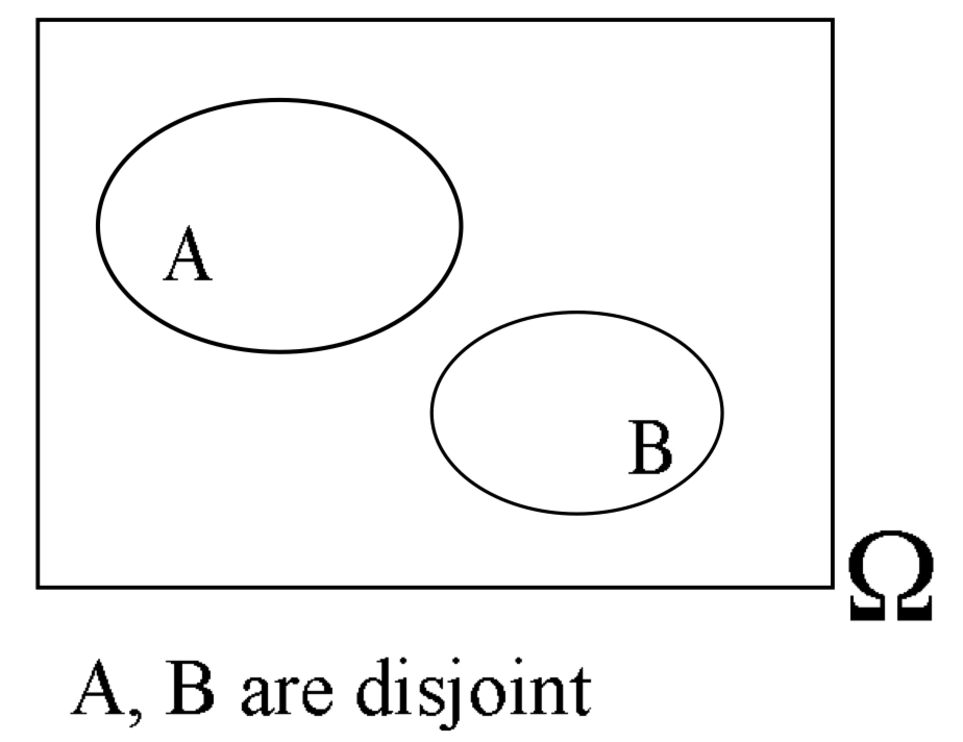
\includegraphics[width=2in]{disjoint.pdf}}

    If $A$ and $B$ are disjoint, their intersection is empty, has 
    therefore probability 0:
    \[
    P(A \cap B) = P(\emptyset) = 0.
    \]
\end{minipage}
\hfill
\begin{minipage}[t]{3.5in}
{\textcolor{cyan}{Independence: }}
    \centerline{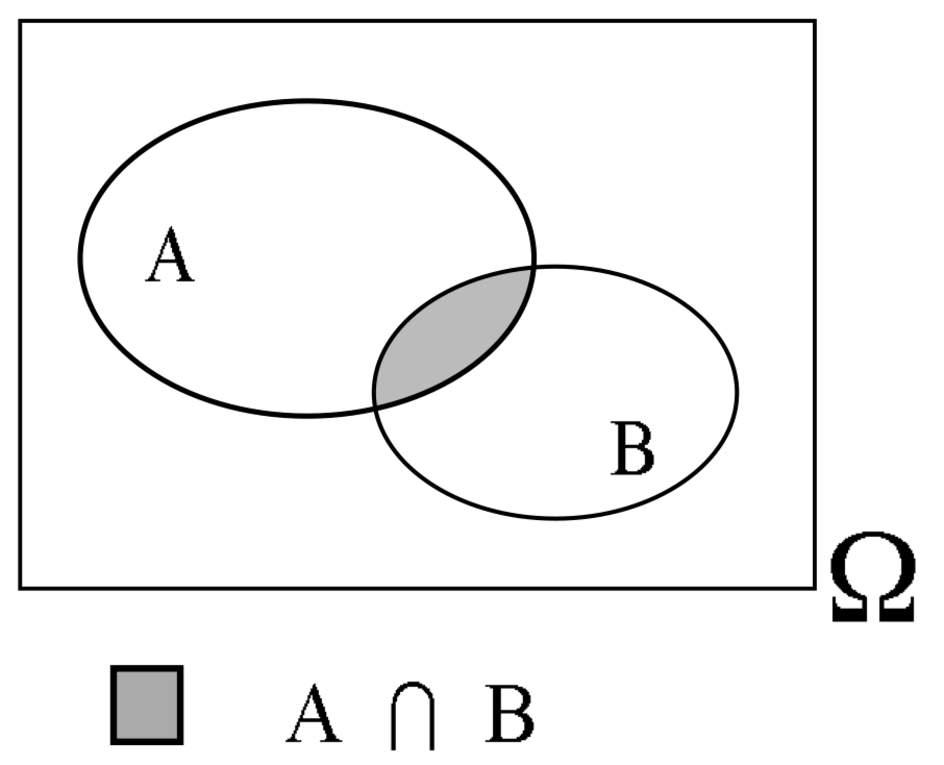
\includegraphics[width=2in]{intersection.pdf}}    
    If $A$ and $B$ are independent events, the probability of their 
    intersection can be computed as the product of their individual 
    probabilities: $P(A \cap B) = P(A) \cdot P(B)$\\[.01in]
    The probability for the intersection is zero only if $A$ or $B$ is empty.
\end{minipage}

\foilhead[-.8in]{\textcolor{blue}{On Systems in Series, Systems in Parallel, and Reliability}}
\no \bul A {\textcolor{magenta}{parallel}} system consists of $k$ components $c_{1}, \ldots, c_{k}$ arranged in such a way that the system works if and only if at least one of the $k$ components functions properly.\\[.1in]
\centerline{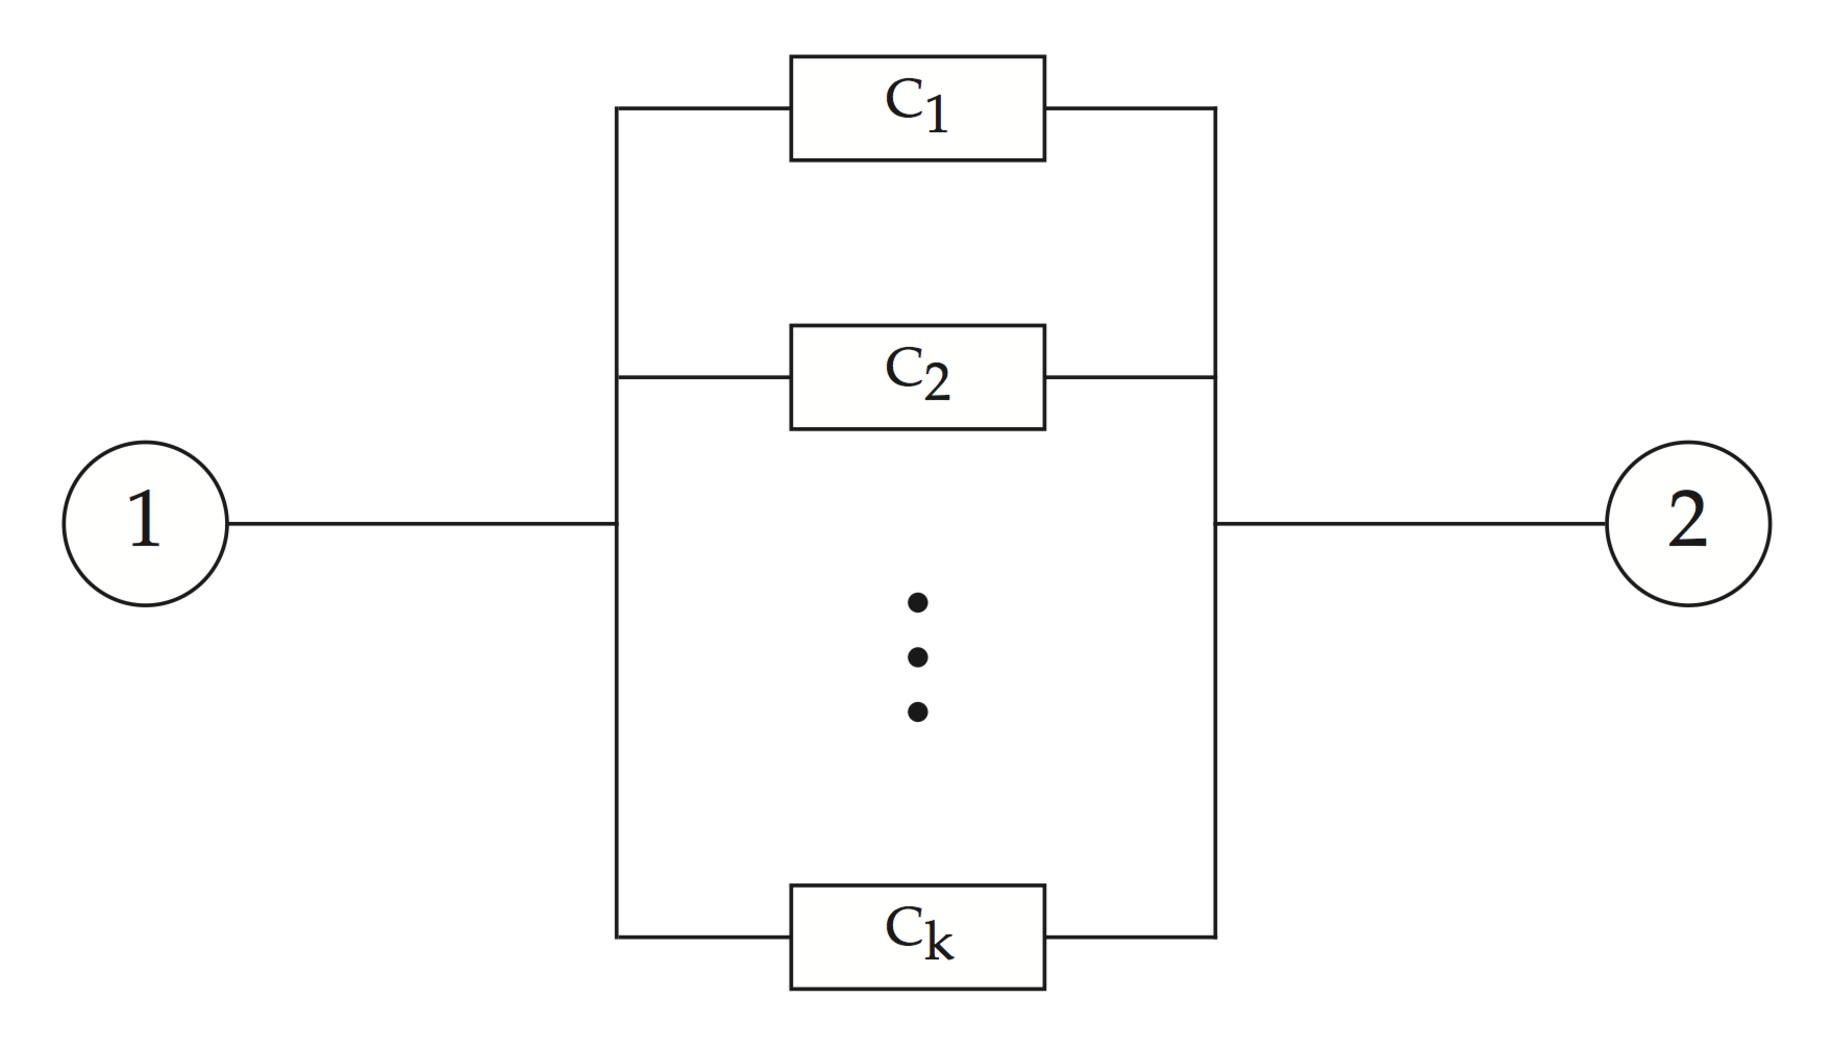
\includegraphics[height=6cm]{parallel-system.pdf}}
\no \bul A {\textcolor{magenta}{serial} system consists of $k$ components $c_{1}, \ldots, c_{k}$ arranged in such a way that the system works if an only if all of the components function properly.\\[.1in]
\centerline{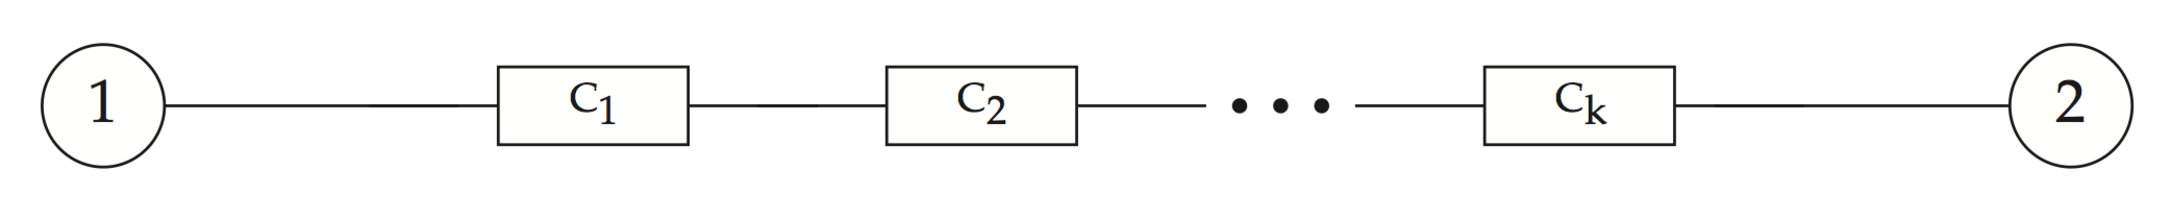
\includegraphics[height=1.5cm]{series-system.pdf}}
\foilhead[-.8in]{\textcolor{blue}{On Systems and Reliability (continued)}}
\begin{itemize}
\item The system consisting of the AOL network and the phone line is an example of a serial system.
\item The {\textcolor{magenta}{reliability}} of a system is the probability that the system works.
\item For example, the reliability of the system consisting of the AOL network and the phone line (if the two are independent) is .54. 
\item We can also construct larger systems with sub-systems that are connected in series and/or in parallel.
\end{itemize}


\foilhead[-.7in]{\textcolor{blue}{Example: Parallel system with $k$ mutually independent components}}
\no {\textcolor{magenta}{Let $c_{1}, \ldots, c_{k}$ denote the $k$ components in a parallel system. Assume the $k$ components operate independently, and $P(c_{j} \text{ works })=p_{j}$. What is the reliability of the system?}}
\begin{eqnarray*}
P(\text{ system works}) &=& P(\text{ at least one component works}) \\
&=& 1-P(\text{ all components fail }) \\ 
&=& 1-P(c_{1} \text{ fails and } c_{2} \text{ fails } \ldots \text{ and } c_{k} \text{ fails }) \\ 
&=& 1- \prod_{j=1}^k P(c_j \text{ fails}) \\
&=& 1- \prod_{j=1}^{k}(1-p_{j}). 
\end{eqnarray*}

\foilhead[-.7in]{\textcolor{blue}{Example: System in series with $k$ mutually independent components}}
%\begin{itemize}
\no {\textcolor{magenta}{Let $c_{1}, \ldots, c_{k}$ denote the $k$ components in a system. Assume the $k$ components are connected in series, operate independently, and $P(c_{j} \text{ works })=p_{j}$. What is the reliability of the system?}}
\begin{eqnarray*}
P(\text{ system works}) &=& P(\text{ all components work}) \\
&=& \prod_{j=1}^k P(c_j \text works) \\
&=& \prod_{j=1}^{k}p_{j}.
\end{eqnarray*}

\foilhead[-.78in]{\textcolor{blue}{Reliability of Systems (continued) }}
\no  {\textcolor{magenta}{Example 2.17:}}{\textcolor{cyan}{Each component in the system shown below is opearable with probability 0.92 independently of other components. Calculate the reliability}} \\[.01in]
\begin{minipage}[t]{4.25in}
{\textcolor{cyan}{of the system:}}\\[.01in]  
\includegraphics*[scale=.25]{circuit1.pdf}\\[.01in]
\no 1. The upper link A-B works if both A and B work.   Thus we can replace this link with a component F that operates with probability $P(A\cap B)=(0.92)^2=0.8464$
\end{minipage}
\hfill
\begin{minipage}[t]{4.25in}
\no 2. The components D and E connected in parallel can be replaced by component G that operates with probability\\ 
$P(D\cup E)=1-(1-0.92)^2$\hfill $=0.9936$\\[.1in]
\includegraphics*[scale=.25]{circuit2.pdf}
\end{minipage}
\foilhead[-.7in]{\textcolor{blue}{Example 2.17 (continued) }}
\no 3. The components C  and G connected in series so they can be replaced by a component H that operates with probability\\[.1in]
\hspace*{2in}$P(C\cap G)=(0.92)(0.9936)=0.9141$\\[.1in]
\hspace*{2.5in}\includegraphics*[scale=.3]{circuit3.pdf}\\[.1in]
\no 4. Lastly, the components F and H are in parallel so the reliability of the system is\\[.1in]
\hspace*{2in}$P(F\cup H)=1-(1-0.8424)(1-0.9141)=0.9868$


\end{document}





